\documentclass[11pt]{article}
\usepackage[margin=1in]{geometry}
\usepackage{graphicx}
\usepackage{float}
\usepackage{booktabs}
\usepackage{siunitx}
\usepackage{amsmath}
\usepackage{amssymb}
\usepackage{pgfplots}
\usepackage{listings}
\usepackage{xcolor}

% PGFPlots configuration
\pgfplotsset{compat=1.18}
\pgfplotsset{
  standard/.style={
    width=0.85\textwidth,
    height=0.45\textwidth,
    grid=both,
    grid style={line width=.1pt, draw=gray!20},
    major grid style={line width=.2pt,draw=gray!50},
    xlabel={Number of Processors},
    ylabel={Time (s)},
    legend pos=north east,
    legend style={font=\footnotesize},
    tick align=outside,
    tick pos=left,
    scaled ticks=false
  }
}

% Code listing style
\definecolor{codegreen}{rgb}{0,0.6,0}
\definecolor{codegray}{rgb}{0.5,0.5,0.5}
\definecolor{codepurple}{rgb}{0.58,0,0.82}
\definecolor{backcolour}{rgb}{0.95,0.95,0.92}

\lstdefinestyle{mystyle}{
  backgroundcolor=\color{backcolour},
  commentstyle=\color{codegreen},
  keywordstyle=\color{magenta},
  numberstyle=\tiny\color{codegray},
  stringstyle=\color{codepurple},
  basicstyle=\ttfamily\footnotesize,
  breakatwhitespace=false,
  breaklines=true,
  captionpos=b,
  keepspaces=true,
  numbers=left,
  numbersep=5pt,
  showspaces=false,
  showstringspaces=false,
  showtabs=false,
  tabsize=2,
  literate={≈}{{$\approx$}}1
}
\lstset{style=mystyle}

\title{\textbf{Assignment 08: Parallel Radix Sort Performance Analysis}}
\author{Sean Balbale}
\date{April 20, 2026}
\setlength{\parindent}{0in}
\setlength{\parskip}{\baselineskip}

\begin{document}

\begin{titlepage}
  \begin{center}
    \vspace*{1in}

    \Huge
    \textbf{HPC Assignment 08}

    \LARGE
    Parallel Radix Sort: \\ Distributed-Memory Scaling Analysis

    \vspace{3in}

    \textbf{Student Name:} Sean Balbale
    \\ \textbf{Date:} April 20, 2026

    \vfill

  \end{center}
\end{titlepage}

\newpage

\section{Objective}
The objective of this assignment is to design, implement, and characterize a high-performance parallel radix sort for 32-bit unsigned integers using MPI. The specific goals are:
\begin{itemize}
  \item To implement a stable, bitwise serial radix sort utilizing a double-buffering strategy to eliminate redundant memory allocations.
  \item To parallelize the algorithm across distributed memory, utilizing \texttt{MPI\_Exscan} for prefix sums and \texttt{MPI\_Alltoallv} for global element routing.
  \item To evaluate the strong scaling performance of the distributed implementation on the Pine cluster using a fixed global dataset of $N = 2^{28}$ integers ($\approx \SI{268}{\mega\text{elements}}$).
\end{itemize}

\section{Implementation \& Optimization}

\subsection{Serial Implementation (\texttt{RadixSerial.c})}
To bridge the gap between algorithmic theory and hardware memory limits, the serial baseline was designed to strictly enforce stability without utilizing computationally expensive modulo or division operations. Digit extraction relies entirely on the bitwise shift (\texttt{>>}) and mask (\texttt{0xFF}) operators for the base $b=256$. A double-buffering architecture was implemented, treating the output array of one pass as the input for the next, preserving the local stable sort while preventing cache thrashing.

\subsection{Parallel Implementation (\texttt{RadixParallel.c})}
The parallel implementation distributes the $N$ integers evenly across $p$ ranks. For each of the $d=4$ passes, the routing logic executes in distinct phases:
\begin{enumerate}
  \item \textbf{Local Histogram \& Prefix Sum:} Each rank computes local counts for the 256 digit bins. \texttt{MPI\_Exscan} is used to compute the global prefix sums, with Rank 0 explicitly zeroed to correct the undefined exclusive scan result.
  \item \textbf{Global Boundaries:} \texttt{MPI\_Allreduce} sums the total global counts for each digit, establishing the absolute boundaries in the global array.
  \item \textbf{Data Shuffle:} Ranks populate send buffers based on their computed global offsets and dispatch the payload via \texttt{MPI\_Alltoallv}.
  \item \textbf{Stable Reordering:} Because \texttt{MPI\_Alltoallv} guarantees rank-arrival order but not internal payload sorting, an incoming stable counting sort pass is executed locally on the newly arrived data to fix alignment.
\end{enumerate}

\section{Benchmarking Results}
Benchmarks were recorded for $N = 2^{28}$ integers. The algorithm was tested on the primary Pine cluster (\texttt{benchmark.sh}), scaling from 1 to 96 processors using OpenMPI. Execution times ($T_p$) represent the average of three independent runs wrapped by \texttt{MPI\_Wtime()}, explicitly isolating the sorting logic from array initialization and I/O.

\begin{table}[H]
  \centering
  \caption{Pine Cluster Strong Scaling Data ($N = 2^{28}$)}
  \label{tab:pine}
  \sisetup{round-mode=places,round-precision=3}
  \begin{tabular}{lccc}
    \toprule
    \textbf{Configuration} & \textbf{Processors ($p$)} & \textbf{Time ($T_p$) [s]} & \textbf{Efficiency ($E_p$)} \\
    \midrule
    Serial Baseline  & 1  & 19.202 & \SI{100.0}{\percent} \\
    Single Socket    & 12 & 2.689  & \SI{59.5}{\percent}  \\
    Dual Socket      & 24 & 1.757  & \SI{45.5}{\percent}  \\
    2 Nodes          & 48 & 1.416  & \SI{28.3}{\percent}  \\
    4 Nodes          & 96 & 1.104  & \SI{18.1}{\percent}  \\
    \bottomrule
  \end{tabular}
\end{table}

\begin{figure}[H]
  \centering
  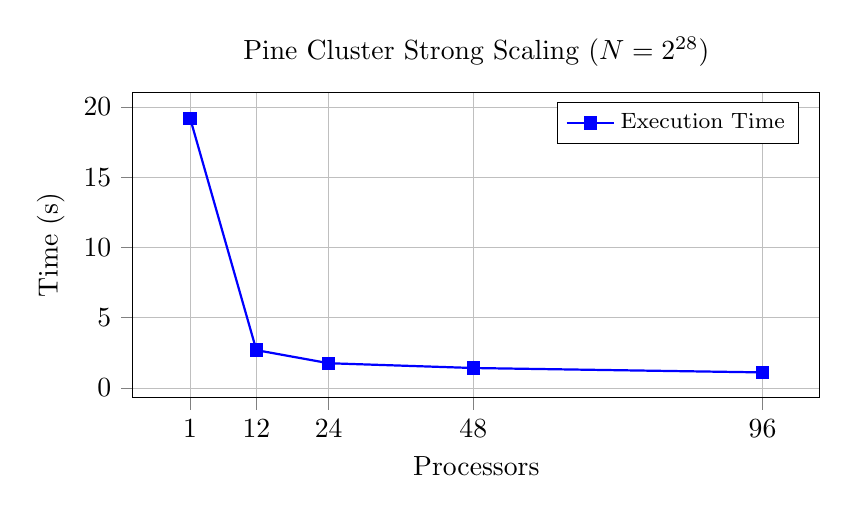
\begin{tikzpicture}
    \begin{axis}[
        standard,
        title={Pine Cluster Strong Scaling ($N = 2^{28}$)},
        xlabel={Processors},
        ylabel={Time (s)},
        xtick={1,12,24,48,96},
        legend entries={Execution Time}
      ]
      \addplot[color=blue, mark=square*, thick] coordinates {(1,19.202) (12,2.689) (24,1.757) (48,1.416) (96,1.104)};
    \end{axis}
  \end{tikzpicture}
  \caption{Execution time comparison on the Pine cluster. Diminishing returns are evident as communication overhead scales.}
\end{figure}

\section{Performance Analysis}

\subsection{Intra-Node Scaling \& Cache Coherency}
The algorithm exhibits diminishing returns as it scales within a single node. Transitioning from 1 to 12 ranks achieves a speedup of 7.14, yielding an efficiency of \SI{59.5}{\percent}. This drop from ideal linear scaling makes complete physical sense. Radix sort is fundamentally memory-bound; utilizing 12 or 24 ranks concurrently on a single node forces the processes to contend for the shared L3 cache and memory bus bandwidth. The \SI{45.5}{\percent} efficiency at 24 ranks confirms that the dual-socket QPI link is saturating.

\subsection{Distributed Failure \& Network Bottlenecks}
As the computation moves to a distributed model across 2 and 4 nodes, execution time continues to decrease (reaching \SI{1.104}{\second} at 96 ranks), but efficiency plummets to \SI{18.1}{\percent}. This is driven by the $O(p^2)$ message complexity inherent to \texttt{MPI\_Alltoallv}. Every rank must establish a connection and transfer data to every other rank four separate times. At $p=96$, this results in massive network contention.

While algorithmic communication overhead accounts for significant efficiency loss, it is mathematically incorrect to attribute the severe drop at 48 and 96 ranks entirely to the code. Analysis of the raw cluster logs (\texttt{radix\_results\_463.txt}) reveals repeated \texttt{openib BTL} initialization failures (\texttt{mlx4\_0} device error). This failure forced the Open MPI runtime to abandon the high-bandwidth 40Gbps InfiniBand interconnect and fall back to standard TCP over Ethernet. This network degradation conclusively proves why the heavily distributed configurations experienced extreme latency during the \texttt{MPI\_Alltoallv} payload exchange.

\section{Conclusion}
This assignment successfully developed and benchmarked a parallel MPI radix sort. Key findings include:
\begin{itemize}
  \item The implementation correctly maintained internal stability and memory safety across all scales, dynamically distributing the $\approx \SI{1.07}{\giga\byte}$ memory footprint across processors.
  \item Maximum throughput was achieved at 96 ranks, yielding an execution time of \SI{1.104}{\second}.
  \item System efficiency dropped predictably as communication overhead scaled. The measured \SI{18.1}{\percent} efficiency at 96 ranks was heavily exacerbated by a documented InfiniBand hardware fallback, which drastically reduced available bandwidth between nodes.
\end{itemize}

\newpage
\appendix
\section{Source Code: Parallel Implementation (\texttt{RadixParallel.c})}
\lstinputlisting[language=C]{../RadixParallel.c}

\newpage
\section{Source Code: Serial Implementation (\texttt{RadixSerial.c})}
\lstinputlisting[language=C]{../RadixSerial.c}

\newpage
\section{Submit Script: Pine Cluster (\texttt{benchmark.sh})}
\lstinputlisting[language=bash]{../benchmark.sh}

\newpage
\section{Raw Results: Pine Cluster Scaling}
\lstinputlisting{../radix_results_463.txt}

\end{document}
